\documentclass[11pt]{article}

\usepackage{latexsym}
\usepackage{amssymb}
\usepackage{amsthm}
\usepackage{graphicx}
\usepackage{enumerate}
\usepackage{amsmath}
\usepackage{cancel}
\numberwithin{equation}{section}

\setlength{\evensidemargin}{.25in}
\setlength{\oddsidemargin}{-.25in}
\setlength{\topmargin}{-.75in}
\setlength{\textwidth}{6.5in}
\setlength{\textheight}{9.5in}
\newcommand{\due}{October 7th, 2015}
\newcommand{\HWnum}{5}
\newcommand{\grad}{\bold\nabla}
\newcommand{\vecE}{\vec{E}}
\newcommand{\scrptR}{\vec{\mathfrak{R}}}
\newcommand{\kapa}{\frac{1}{4\pi\epsilon_0}}
\newcommand{\emf}{\mathcal{E}}
\newcommand{\unit}[1]{\ensuremath{\, \mathrm{#1}}}
\newcommand{\real}{\textnormal{Re}}
\newcommand{\Erf}{\textnormal{Erf}}
\newcommand{\sech}{\textnormal{sech}}
\newcommand{\scrO}{\mathcal{O}}
\newcommand{\levi}{\widetilde{\epsilon}}
\newcommand{\partiald}[2]{\ensuremath{\frac{\partial{#1}}{\partial{#2}}}}
\newcommand{\norm}[2]{\langle{#1}|{#2}\rangle}
\newcommand{\inprod}[2]{\langle{#1}|{#2}\rangle}
\newcommand{\ket}[1]{|{#1}\rangle}
\newcommand{\bra}[1]{\langle{#1}|}





\begin{document}
\begin{titlepage}
\setlength{\topmargin}{1.5in}
\begin{center}
\Huge{Physics 3320} \\
\LARGE{Principles of Electricity and Magnetism II} \\
\Large{Professor Ana Maria Rey} \\[1cm]

\huge{Homework \#\HWnum}\\[0.5cm]

\large{Joe Becker} \\
\large{SID: 810-07-1484} \\
\large{\due} 

\end{center}

\end{titlepage}



\section{Problem \#1}
\begin{enumerate}[(a)]
\item We note \emph{Noether's Theorem} which states that for every symmetry in the action
there exists a conserved quantity. We can use this theorem to find the conserved quantity 
that corresponds to the symmetry due to the Lagrangian's invariance under a translation
$\mathbf{r'} = \mathbf{r}+\epsilon\mathbf{s}$. This translation transforms our generalized 
coordinates by
$$q_i \rightarrow q_i' = q_i+\epsilon s_i$$
where the time derivative of $q_i$ is
$$\dot{q}_i \rightarrow \dot{q}_i' = \dot{q}_i+\epsilon \dot{s}_i$$
We can define the difference between the Lagrangian between the two generalized coordinates
as a quantity 
$$\delta{L} \equiv L(q_i',\dot{q}_i',t) - L(q_i,\dot{q}_i)$$
we note that $\delta{L}=0$ by the assumption that the Lagrangian is invariant under 
translation. So we expand $L(q_i',\dot{q}_i',t)$ by noting that $q_i'=q_i+\epsilon s_i$ where
$\epsilon$ is small so we are able to expand about the point $q_i$ with a perturbation 
$\epsilon s_i$. This yields
$$L(q_i',\dot{q}_i',t) = L(q_i,\dot{q}_i,t) + \partiald{L}{q_i}\epsilon{s_i} + \partiald{L}{\dot{q}_i}\epsilon\dot{s}_i$$
So we see the $\delta{L}$ becomes
\begin{align*}
\delta{L} &= L(q_i',\dot{q}_i',t) - L(q_i,\dot{q}_i)\\
&\Downarrow\\
\delta{L} = 0 &=\cancel{L(q_i,\dot{q}_i,t)} + \partiald{L}{q_i}\epsilon{s_i} + \partiald{L}{\dot{q}_i}\epsilon\dot{s}_i - \cancel{L(q_i,\dot{q}_i)}\\
0 &= \partiald{L}{q_i}\epsilon{s_i} + \partiald{L}{\dot{q}_i}\epsilon\dot{s}_i \\
0 &= \partiald{L}{q_i}s_i + \partiald{L}{\dot{q}_i}\dot{s}_i 
\end{align*}
Next we need to use the \emph{generalized momentum} which is defined by 
$$p_i = \partiald{L}{\dot{q}_i}$$
where we note that the time derivative of the generalized momentum is
$$\frac{dp_i}{dt} = \partiald{L}{q_i}$$
So we see that we have
\begin{align*}
0 &= \partiald{L}{q_i}s_i + \partiald{L}{\dot{q}_i}\dot{s}_i\\
&\Downarrow\\
0 &= \frac{dp_i}{dt}s_i + p_i\frac{ds_i}{dt}\\
0 &= \frac{d}{dt}p_is_i = \frac{d}{dt}\left(\mathbf{p}\cdot\mathbf{s}\right)
\end{align*}
So we see the quantity $\mathbf{p}\cdot\mathbf{s}$ is conserved. This corresponds to the 
conservation of linear momentum.

\item Next we repeat the process for a perturbation in a rotation given by
$$\mathbf{r}' = \mathbf{r}+\epsilon\mathbf{s}\times\mathbf{r}$$
This yields a generalized coordinate 
$$r_i' = r_i + \epsilon(\mathbf{s}\times\mathbf{r})_i$$
with the time derivative given by
$$\dot{r}_i' = \dot{r}_i + \epsilon\frac{d}{dt}(\mathbf{s}\times\mathbf{r})_i$$
Following the same logic as in part (a) we have
\begin{align*}
\delta{L} = 0 &= \partiald{L}{r_i}\epsilon(\mathbf{s}\times\mathbf{r})_i + \partiald{L}{\dot{r}_i}\epsilon\frac{d}{dt}(\mathbf{s}\times\mathbf{r})_i\\
&\Downarrow\\
0 &= \frac{dp_i}{dt}(\mathbf{s}\times\mathbf{r})_i + p_i\frac{d}{dt}(\mathbf{s}\times\mathbf{r})_i\\
0 &= \frac{d}{dt}p_i(\mathbf{s}\times\mathbf{r})_i \\
0 &= \frac{d}{dt}\mathbf{p}\cdot(\mathbf{s}\times\mathbf{r}) \\
0 &= \frac{d}{dt}\mathbf{s}\cdot(\mathbf{r}\times\mathbf{p}) \\
0 &= \frac{d}{dt}\mathbf{s}\cdot\mathbf{L}
\end{align*}
Note we defined the angular momentum by $\mathbf{L} = \mathbf{r}\times\mathbf{p}$ So the 
quantity $\mathbf{s}\cdot\mathbf{L}$ is conserved. This corresponds to the conservation of
angular momentum.

\item For the Lagrangian for $N$-particles in 3D
$$L = \sum_{i=1}^{N}\frac{1}{2}m_i\mathbf{v}_i\cdot\mathbf{v}_i - \sum_{i<j}V\left(|\mathbf{r}_i-\mathbf{r}_j|\right)$$
under a uniform translation 
$$\mathbf{r}_i' = \mathbf{r}_i+\epsilon\mathbf{s}$$
we see that the potential term remains invariant because it is only dependent on the 
relative position between particles. Next we note that the vector $\mathbf{s}$ is constant 
so we have
$$\dot{\mathbf{r}}_i' = \dot{\mathbf{r}}_i.$$
We see that the kinetic energy does not depend on the position so we can easily see that
the Lagrangian is invariant. This corresponds to the conservation of energy.
\end{enumerate}

\pagebreak

\section{Problem \#2}
\begin{figure}
\centering
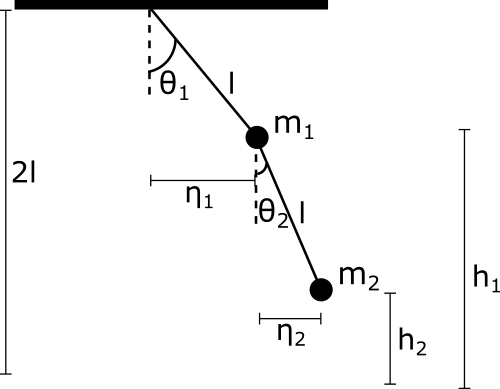
\includegraphics[width=0.8\textwidth]{figure.png}
\caption{The double pendulum system with labeled lengths and masses.}
\label{figure}
\end{figure}
\begin{enumerate}[(a)]
\item For a double pendulum with equal lengths, $l$, and different masses $m_1$ and $m_2$ as
shown in Figure \ref{figure}. We can use this geometry and the assumption of small 
oscillations. This allows us to use the transverse displacements from vertical, $\eta_1$ and 
$\eta_2$, as the generalized coordinates for the Lagrangian. We see that the displacements 
are given by
$$\eta_1 = l\sin\theta_1= l\theta_1+\scrO(\theta_1^3);\qquad \eta_2=l\sin\theta_2= l\theta_2+\scrO(\theta_2^3)$$
We also can see that the displacement for $m_2$ we have to account for the displacement from
the pivot point which is $\eta_1+\eta_2$. Using this we can say the kinetic energy is given 
by
$$T = \frac{1}{2}m_1\dot{\eta}_1^2 + \frac{1}{2}m_2\left(\dot{\eta}_1+\dot{\eta}_2\right)^2$$
In order to determine the potential we note that it is given by
$$V = m_1gh_1+m_2gh_2$$
where we need to find $h_1$ and $h_2$ in our generalized coordinates by expanding about 
$\theta_1$
\begin{align*}
h_1 &= 2l-l\cos\theta_1\\
&= l\left(2-1+\frac{1}{2}\theta_1^2+\scrO(\theta_1^3)\right)\\
&= l\left(1+\frac{1}{2}\frac{\eta_1^2}{l^2}\right)
\end{align*}
And for $h_2$ we find
\begin{align*}
h_2 &= 2l-l\cos\theta_1-l\cos\theta_2\\
&= l\left(2-1+\frac{1}{2}\theta_1^2-1+\frac{1}{2}\theta_2^2+\scrO(\theta_1^3,\theta_2^3)\right)\\
&= \frac{l}{2}\left(\theta_1^2+\theta_2^2\right)\\
&= \frac{l}{2}\left(\frac{\eta_1^2}{l^2}+\frac{\eta_2^2}{l^2}\right)\\
&= \frac{1}{2l}\left(\eta_1^2+\eta_2^2\right)\\
\end{align*}
So we can write the potential in terms of $\eta_1$ and $\eta_2$ as
\begin{align*}
V &= m_1gh_1+m_2gh_2\\
&\Downarrow\\
V &= m_1gl\left(1+\frac{1}{2}\frac{\eta_1^2}{l^2}\right)+m_2g\frac{1}{2l}\left(\eta_1^2+\eta_2^2\right)\\
&= m_1gl + \frac{m_1g\eta_1^2}{2l} + \frac{m_2g\eta_1^2}{2l} + \frac{m_2g\eta_2^2}{2l}\\
&= \frac{g}{2l}\left(m_1\eta_1^2 + m_2\eta_1^2 + m_2\eta_2^2\right)\\
&= \frac{g}{2l}\left((m_1 + m_2)\eta_1^2 + m_2\eta_2^2\right)
\end{align*}
Note that we neglected the constant term $m_1gl$ in the potential as we can shift to a new
equilibrium point without loss of generality. So we have the Lagrangian as
\begin{align*}
L &= T - V\\
&\Downarrow\\
L &= \frac{1}{2}m_1\dot{\eta}_1^2 + \frac{1}{2}m_2\left(\dot{\eta}_1+\dot{\eta}_2\right)^2 - \frac{g}{2l}\left((m_1 + m_2)\eta_1^2 + m_2\eta_2^2\right)
\end{align*}

\item In order to calculate the normal frequencies of the double pendulum. We first write the
kinetic energy in the form
$$T = \frac{1}{2}\dot{\eta}_{i}M_{ij}\dot{\eta}_{j}$$
Where $M_{ij}$ is a mass matrix that is by noting that
\begin{align*}
T &= \frac{1}{2}m_1\dot{\eta}_1^2 + \frac{1}{2}m_2\left(\dot{\eta}_1+\dot{\eta}_2\right)^2\\
&\Downarrow\\
&= \frac{1}{2}\left(m_1\dot{\eta}_1^2 + m_2\dot{\eta}_1^2 + m_2\dot{\eta}_2^2 + m_2\dot{\eta}_1\dot{\eta}_2 + m_2\dot{\eta}_2\dot{\eta}_1\right)\\
&= \frac{1}{2}\left((m_1+m_2)\dot{\eta}_1\dot{\eta}_1 + m_2\dot{\eta}_2\dot{\eta}_2 + m_2\dot{\eta}_1\dot{\eta}_2 + m_2\dot{\eta}_2\dot{\eta}_1\right)
\end{align*}
Which implies that
$$M_{ij} = \left(\begin{array}{cc}
                m_1+m_2          &m_2\\
                m_2              &m_2
           \end{array}\right)$$
Next, we need to write the potential energy in the form
$$V = \frac{1}{2}\eta_iV_{ij}\eta_j$$
where we can see that the potential matrix is given by
$$V_{ij} = \left(\begin{array}{cc}
                \dfrac{g(m_1+m_2)}{l}        &0\\
                0              &\dfrac{gm_2}{l}
           \end{array}\right)$$
So, the Lagrangian becomes
$$L = \frac{1}{2}\dot{\eta}_{i}M_{ij}\dot{\eta}_{j} - \frac{1}{2}\eta_iV_{ij}\eta_j$$
where if we find the equations of motion by
\begin{align*}
\frac{d}{dt}\left(\partiald{L}{\dot{\eta}_i}\right) &= \partiald{L}{\eta_i}\\
&\Downarrow\\
\frac{d}{dt}\left(M_{ij}\dot{\eta}_{j}\right) &= -V_{ij}\eta_{j}\\
&\Downarrow\\
M_{ij}\ddot{\eta}_{j} &= -V_{ij}\eta_{j}
\end{align*}
We complexify the solution by 
$$\eta_{j} = A_je^{i\omega{t}}$$
which gives us 
\begin{align*}
\ddot{\eta}_{j} &= -\omega^2A_je^{i\omega{t}}\\
&\Downarrow\\
\ddot{\eta}_{j} &= -\omega^2\eta_{j}
\end{align*}
So we can see that out equation of motion becomes
\begin{align*}
M_{ij}\ddot{\eta}_{j} + V_{ij}\eta_{j} &= 0\\
&\Downarrow\\
M_{ij}(-\omega^2)\eta_{j} + V_{ij}\eta_{j} &= 0\\
\left(V_{ij}-\omega^2M_{ij}\right)A_j\cancel{e^{i\omega{t}}} &= 0\\
\left(V_{ij}-\omega^2M_{ij}\right)A_j &= 0
\end{align*}
So we have two equations for the free index $i$ by $i=1,2$. So for $i=1$ we have the sum
\begin{align*}
\left(V_{1j}-\omega^2M_{1j}\right)A_j &= 0\\
&\Downarrow\\
\left(V_{11}-\omega^2M_{11}\right)A_1 + \left(\cancelto{0}{V_{12}}-\omega^2M_{12}\right)A_2 &= 0\\
&\Downarrow\\
\left(\frac{g(m_1+m_2)}{l}-\omega^2(m_1+m_2)\right)A_1 - \left(\omega^2m_2\right)A_2 &= 0
\end{align*}
Which we can use to get a ratio between $A_1$ and $A_2$ as
$$\frac{A_1}{A_2} =  \frac{m_2}{m_1+m_2}\frac{\omega^2}{\dfrac{g}{l}-\omega^2}$$
And for $i=2$ we have
\begin{align*}
\left(V_{2j}-\omega^2M_{2j}\right)A_j &= 0\\
&\Downarrow\\
\left(\cancelto{0}{V_{21}}-\omega^2M_{21}\right)A_1 + \left(V_{22}-\omega^2M_{22}\right)A_2 &= 0\\
-\left(\omega^2m_2\right)A_1 + \left(\frac{gm_2}{l}-\omega^2m_2\right)A_2 &= 0\\
&\Downarrow\\
\left(\omega^2m_2\right)A_1 &= \left(\frac{gm_2}{l}-\omega^2m_2\right)A_2\\
&\Downarrow\\
\frac{A_1}{A_2} &= \frac{\dfrac{g}{l}-\omega^2}{\omega^2}
\end{align*}
Now we can solve for the normal frequencies by solving
\begin{align*}
\frac{m_2}{m_1+m_2}\frac{\omega^2}{\dfrac{g}{l}-\omega^2} &= \frac{\dfrac{g}{l}-\omega^2}{\omega^2}\\
&\Downarrow\\
(\gamma\omega^2)^2 &= (\dfrac{g}{l}-\omega^2)^2\\
\pm\gamma\omega^2 &= \dfrac{g}{l}-\omega^2\\
\omega^2\pm\gamma\omega^2 &= \dfrac{g}{l}\\
\omega^2(1\pm\gamma) &= \dfrac{g}{l}\\
&\Downarrow\\
\omega^2_{\pm} &= \dfrac{g}{l}(1\pm\gamma)^{-1}
\end{align*}
Note we defined the quantity $\gamma$ as
$$\gamma^2 = \frac{m_2}{m_1+m_2}$$

\item We can construct the normal-mode eigenvectors by noting for the normal frequency
$$\omega^2 = \dfrac{g}{l}(1+\gamma)^{-1}$$
we have the ratio between $A_1$ and $A_2$ as
\begin{align*}
\frac{A_1}{A_2} &= \frac{\dfrac{g}{l}-\omega^2}{\omega^2}\\
&\Downarrow\\
&= \frac{\cancel{\dfrac{g}{l}}-\cancel{\dfrac{g}{l}}\dfrac{1}{1+\gamma}}{\cancel{\dfrac{g}{l}}\dfrac{1}{1+\gamma}}\\
&= \left(1-\frac{1}{1+\gamma}\right)(1+\gamma)\\
&= 1+\gamma - 1 = \gamma
\end{align*}
So this implies that $A_1 = \gamma{A_2}$. Then by $\omega^2_{-}$ we have
\begin{align*}
\frac{A_1}{A_2} &= \frac{\dfrac{g}{l}-\omega^2}{\omega^2}\\
&\Downarrow\\
&= \left(1-\frac{1}{1-\gamma}\right)(1-\gamma)\\
&= 1-\gamma - 1 = -\gamma
\end{align*}
So we have $A_1 = -\gamma{A_2}$. So we have the normal-mode eigenvectors 
$$\vec{\eta}_{\pm} = A_{\pm}\left(\begin{array}{c} 1\\ \pm\gamma^{-1}\end{array}\right)e^{i\omega_{\pm}t}$$
We can note the limiting cases where $m_1\rightarrow{0}$ which is the case of a single 
pendulum of length $2l$ we see that for this limit $\gamma$ becomes
$$\lim_{m_1\rightarrow{0}}\gamma = \lim_{m_1\rightarrow{0}}\frac{m_2}{m_1+m_2} = 1$$
Which yields only a single normal frequency given by
$$\omega^2=\frac{g}{2l}$$
which is as we expect is the frequency of a pendulum with a length of $2l$. In the other 
limit as $m_2\rightarrow{0}$ we note that the system becomes a single pendulum, but of 
length $l$. It is easy to see that 
$$\lim_{m_2\rightarrow{0}}\gamma=0$$
Which makes for a single normal mode frequency given by
$$\omega^2=\frac{g}{l}$$
which is what we expect.

\item We can calculate the modal matrix, $\mathbf{A}$, by first writing $A_{\pm}$ as a 
complex number $A_{\pm} = \rho_{\pm}e^{i\phi_{\pm}}$ which makes the normal eigenmodes become
$$\vec{\eta}_{\pm} = \rho_{\pm}\left(\begin{array}{c} 1\\ \pm\gamma^{-1}\end{array}\right)e^{i(\omega_{\pm}t+\phi_{\pm})}$$
This allows us to normalize the eigenvectors to the mass matrix $M_{ij}$ by
\begin{align*}
1 &= \rho_+(1,\gamma^{-1})\left(\begin{array}{cc}
                m_1+m_2          &m_2\\
                m_2              &m_2
           \end{array}\right)\left(\begin{array}{c}1\\ \gamma^{-1}\end{array}\right)\rho_+\\
&= \rho_+^2(m_1+m_2)(1,\gamma^{-1})\left(\begin{array}{cc}
                1             &\gamma^2\\
                \gamma^2      &\gamma^2
           \end{array}\right)\left(\begin{array}{c}1\\ \gamma^{-1}\end{array}\right)\\
&= \rho_+^2(m_1+m_2)(1,\gamma^{-1})\left(\begin{array}{c}
                1+\gamma\\
                \gamma+\gamma^2 
           \end{array}\right)\\
&= \rho_+^2(m_1+m_2)(1+\gamma+1+\gamma)\\
&= 2\rho_+^2(m_1+m_2)(1+\gamma)\\
&= 2\rho_+^2m_1\frac{1+\gamma}{1-\gamma^2}\\
&= 2\rho_+^2m_1\frac{1+\gamma}{(1+\gamma)(1-\gamma)}\\
&= 2\rho_+^2m_1\frac{1}{1-\gamma}\\
&\Downarrow\\
\rho_+ &= \sqrt{\frac{1-\gamma}{2m_1}}
\end{align*}
Note that we used the fact that $m_1/(m_1+m_2) = 1-\gamma^2$. Now for $\rho_-$
\begin{align*}
1 &= \rho_-^2(m_1+m_2)(1,-\gamma^{-1})\left(\begin{array}{cc}
                1             &\gamma^2\\
                \gamma^2      &\gamma^2
           \end{array}\right)\left(\begin{array}{c}1\\ -\gamma^{-1}\end{array}\right)\\
&= \rho_-^2(m_1+m_2)(1,-\gamma^{-1})\left(\begin{array}{c}
                1-\gamma\\
                \gamma^2-\gamma 
           \end{array}\right)\\
&= \rho_-^2(m_1+m_2)(1-\gamma+1-\gamma)\\
&= 2\rho_-^2(m_1+m_2)(1-\gamma)\\
&\Downarrow\\
\rho_- &= -\sqrt{\frac{1+\gamma}{2m_1}}
\end{align*}
Note that we choose the negative solution though either are valid. Now that we have normalized eigenvectors we can construct $\mathbf{A}$ by
$$\mathbf{A} = \left(p_+\left(\begin{array}{c}1\\ \gamma^{-1}\end{array}\right)
                    \quad p_-\left(\begin{array}{c}1\\ -\gamma^{-1}\end{array}\right)\right) 
= \frac{1}{\sqrt{2m_1}}\left(\begin{array}{cc} 
                         (1-\gamma)^{1/2}          &-(1+\gamma)^{1/2}\\
                         \gamma^{-1}(1-\gamma)^{1/2}    &\gamma^{-1}(1+\gamma)^{1/2}\\
\end{array}\right)$$
Now we can demonstrate that $\mathbf{A}$ diagonalizes the mass matrix by
\begin{align*}
\mathbf{A}^T\mathbf{M}\mathbf{A} &= \frac{m_1+m_2}{2m_1}
                     \left(\begin{array}{cc} 
                         (1-\gamma)^{1/2}          &\gamma^{-1}(1-\gamma)^{1/2}\\
                         -(1+\gamma)^{1/2}         &\gamma^{-1}(1+\gamma)^{1/2}\\
                      \end{array}\right)
                      \left(\begin{array}{cc}
                         1             &\gamma^2\\
                         \gamma^2      &\gamma^2
                     \end{array}\right)
                    \left(\begin{array}{cc} 
                         (1-\gamma)^{1/2}          &-(1+\gamma)^{1/2}\\
                         \gamma^{-1}(1-\gamma)^{1/2}    &\gamma^{-1}(1+\gamma)^{1/2}\\
                     \end{array}\right)\\
&= \frac{m_1+m_2}{2m_1}
                     \left(\begin{array}{cc} 
                         (1-\gamma)^{1/2}          &\gamma^{-1}(1-\gamma)^{1/2}\\
                         -(1+\gamma)^{1/2}         &\gamma^{-1}(1+\gamma)^{1/2}\\
                      \end{array}\right)
                      \left(\begin{array}{cc}
                          (1-\gamma)^{1/2}(1+\gamma)           &(1+\gamma)^{1/2}(\gamma-1)\\ 
                          \gamma(1-\gamma)^{1/2}(1+\gamma)     &-\gamma(1+\gamma)^{1/2}(\gamma-1)\\ 
                      \end{array}\right)\\
&= \frac{m_1+m_2}{2m_1}
                     \left(\begin{array}{cc} 
                         2(1-\gamma^2)                  &0\\
                         0                              &2(1-\gamma^2)
                      \end{array}\right)\\
&= \frac{1}{2(1-\gamma^2)}2(1-\gamma^2)\mathbf{I} = \mathbf{I}
\end{align*}
So as we expect we obtain the identity matrix, $\mathbf{I}$. Now for the potential matrix we
calculate
\begin{align*}
\mathbf{A}^T\mathbf{V}\mathbf{A} &= \frac{g(m_1+m_2)}{2lm_1}
                     \left(\begin{array}{cc} 
                         (1-\gamma)^{1/2}          &\gamma^{-1}(1-\gamma)^{1/2}\\
                         -(1+\gamma)^{1/2}         &\gamma^{-1}(1+\gamma)^{1/2}\\
                      \end{array}\right)
                      \left(\begin{array}{cc}
                         1             &0\\
                         0             &\gamma^2
                     \end{array}\right)
                    \left(\begin{array}{cc} 
                         (1-\gamma)^{1/2}          &-(1+\gamma)^{1/2}\\
                         \gamma^{-1}(1-\gamma)^{1/2}    &\gamma^{-1}(1+\gamma)^{1/2}
                     \end{array}\right)\\
&= \frac{g}{2l(1-\gamma^2)}
                     \left(\begin{array}{cc} 
                         (1-\gamma)^{1/2}          &\gamma^{-1}(1-\gamma)^{1/2}\\
                         -(1+\gamma)^{1/2}         &\gamma^{-1}(1+\gamma)^{1/2}
                      \end{array}\right)
                      \left(\begin{array}{cc}
                         (1-\gamma)^{1/2}                   &-(1-\gamma)^{1/2}\\
                         \gamma(1-\gamma)^{1/2}             &\gamma(1+\gamma)^{1/2}
                     \end{array}\right)\\
&= \frac{g}{2l(1-\gamma^2)}
                     \left(\begin{array}{cc} 
                         2(1-\gamma)          &0\\
                         0                    &2(1+\gamma)\\
                      \end{array}\right)\\
&= \frac{g}{l}
                     \left(\begin{array}{cc} 
                         (1+\gamma)^{-1}          &0\\
                         0                         &(1-\gamma)^{-1}\\
                      \end{array}\right)\\
&= \left(\begin{array}{cc} 
                         \omega_+^2         &0\\
                         0                  &\omega_-^2
                      \end{array}\right)
\end{align*}
We see that as we expect we get the diagonalized matrix contains the normal frequencies.

\item We can use the modal matrix, $\mathbf{A}$, to construct the normal coordinates, 
$\xi(t)$ by
$$\xi(t) = \mathbf{A}^T\mathbf{M}\vec{\eta}(t)$$
Where we take $\vec{\eta}(t)$ as the general solution given by the linear combination 
$$\vec{\eta}(t) = \textnormal{Re}(C_+\vec{\eta}_{+}(t)+C_-\vec{\eta}_{-}(t))$$
This linear combination is projecting the generalized coordinates $\eta_1$ and $\eta_2$ into
the basis of the normal eigenmodes which form an orthonormal basis by the above work. So we 
can calculate
\begin{align*}
C_+\eta_{+}(t)+C_-\eta_{-}(t) &= C_+\rho_+\left(\begin{array}{c} 1\\ \gamma^{-1}\end{array}\right)e^{i(\omega_{+}t+\phi_{+})}
+C_-\rho_{-}\left(\begin{array}{c} 1\\ \pm\gamma^{-1}\end{array}\right)e^{i(\omega_{-}t+\phi_{-})}\\
&= \frac{1}{\sqrt{2m_1}}\left(\begin{array}{c} 
                C_+(1-\gamma)^{1/2}e^{i(\omega_{+}t+\phi_{+})}\\ 
                C_+\gamma^{-1}(1-\gamma)^{1/2}e^{i(\omega_{+}t+\phi_{+})}
                       \end{array}\right)
+ \frac{1}{\sqrt{2m_1}}\left(\begin{array}{c} 
                -C_-(1+\gamma)^{1/2}e^{i(\omega_{-}t+\phi_{-})}\\ 
                C_-\gamma^{-1}(1+\gamma)^{1/2}e^{i(\omega_{-}t+\phi_{-})}
                       \end{array}\right)\\
&= \frac{1}{\sqrt{2m_1}}\left(\begin{array}{c} 
                C_+(1-\gamma)^{1/2}e^{i(\omega_{+}t+\phi_{+})}-C_-(1+\gamma)^{1/2}e^{i(\omega_{-}t+\phi_{-})}\\ 
                C_+\gamma^{-1}(1-\gamma)^{1/2}e^{i(\omega_{+}t+\phi_{+})}+C_-\gamma^{-1}(1+\gamma)^{1/2}e^{i(\omega_{-}t+\phi_{-})}
                       \end{array}\right)\\
&= \frac{1}{\sqrt{2m_1}}\left(\begin{array}{c} 
                C_+(1-\gamma)^{1/2}\cos(\omega_{+}t+\phi_{+})-C_-(1+\gamma)^{1/2}\cos(\omega_{-}t+\phi_{-})\\ 
                C_+\gamma^{-1}(1-\gamma)^{1/2}\cos(\omega_{+}t+\phi_{+})+C_-\gamma^{-1}(1+\gamma)^{1/2}\cos(\omega_{-}t+\phi_{-})
                       \end{array}\right)
\end{align*}

So we calculate $\vec{\xi}$ as 
\begin{align*}
\vec{\xi}(t) &= \mathbf{A}^T\mathbf{M}\vec{\eta}_{+}(t)\\
&=\frac{m_1+m_2}{2m_1}
    \left(\begin{array}{cc} 
         (1-\gamma)^{1/2}          &\gamma^{-1}(1-\gamma)^{1/2}\\
         -(1+\gamma)^{1/2}         &\gamma^{-1}(1+\gamma)^{1/2}\\
     \end{array}\right)
     \left(\begin{array}{cc}
        1             &\gamma^2\\
        \gamma^2      &\gamma^2
    \end{array}\right)\\
&\qquad\times    \left(\begin{array}{c} 
         C_+(1-\gamma)^{1/2}\cos(\omega_{+}t+\phi_{+})-C_-(1+\gamma)^{1/2}\cos(\omega_{-}t+\phi_{-})\\ 
         C_+\gamma^{-1}(1-\gamma)^{1/2}\cos(\omega_{+}t+\phi_{+})+C_-\gamma^{-1}(1+\gamma)^{1/2}\cos(\omega_{-}t+\phi_{-})
    \end{array}\right)\\
&=\frac{1}{2(1-\gamma^2)}
    \left(\begin{array}{cc} 
         (1+\gamma)(1-\gamma)^{1/2}          &\gamma(1+\gamma)(1-\gamma)^{1/2}\\
         (-1+\gamma)(1+\gamma)^{1/2}         &\gamma(1-\gamma)(1+\gamma)^{1/2}
     \end{array}\right)\\
&\qquad\times    \left(\begin{array}{c} 
         C_+(1-\gamma)^{1/2}\cos(\omega_{+}t+\phi_{+})-C_-(1+\gamma)^{1/2}\cos(\omega_{-}t+\phi_{-})\\ 
         C_+\gamma^{-1}(1-\gamma)^{1/2}\cos(\omega_{+}t+\phi_{+})+C_-\gamma^{-1}(1+\gamma)^{1/2}\cos(\omega_{-}t+\phi_{-})
    \end{array}\right)\\
&=\frac{1}{2(1-\gamma^2)}
    \left(\begin{array}{c} 
         2C_+(1-\gamma)(1+\gamma)\cos(\omega_{+}t+\phi_{+})\\
         2C_-(1-\gamma)(1+\gamma)\cos(\omega_{-}t+\phi_{-})
    \end{array}\right)\\
&= \left(\begin{array}{c} 
         C_+\cos(\omega_{+}t+\phi_{+})\\
         C_-\cos(\omega_{-}t+\phi_{-})
    \end{array}\right)
\end{align*}

\item Now in the limiting case where $m_2<<m_1$ where $\eta_1$ is slightly displaced we have 
the initial conditions 
$$\eta_1(0) = \delta; \qquad \eta_2(0) = 0; \qquad \dot{\eta}_{1}(0)=\dot{\eta}_{1}(0)=0$$
Applying these initial conditions to $\vec{\xi}(t)$ to determine our coefficients by noting 
that 
$$\vec{\eta}(t) = A\vec{\xi}(t)$$
So we apply the initial condition
\begin{align*}
\dot{\vec{\eta}}(0) &= A\dot{\vec{\xi}}(0)\\
&\Downarrow\\
            \sqrt{2m_1}\mathbf{A}^{-1}\left(\begin{array}{c}
                 0\\
                 0
                  \end{array}\right)
&=                 \left(\begin{array}{c}
                    C_+\omega_+\sin(\omega_{+}0+\phi_{+})\\
                    C_-\omega_-\sin(\omega_{-}0+\phi_{-})
                  \end{array}\right)\\
&\Downarrow\\
            \left(\begin{array}{c}
                 0\\
                 0
                  \end{array}\right)
&=                 \left(\begin{array}{c}
                    C_+\omega_+\sin(\phi_{+})\\
                    C_-\omega_-\sin(\phi_{-})
                  \end{array}\right)\\
&\Downarrow\\
\phi_+ = 0&\qquad\phi_-=0
\end{align*}
Now we can apply the initial condition on $\vec{\eta}$
\begin{align*}
\vec{\eta}(0) &= A\vec{\xi}(0)\\
&\Downarrow\\
            \left(\begin{array}{c}
                 \delta\\
                 0
                  \end{array}\right)
&= \frac{1}{\sqrt{2m_1}}\left(\begin{array}{cc} 
                         (1-\gamma)^{1/2}          &-(1+\gamma)^{1/2}\\
                         \gamma^{-1}(1-\gamma)^{1/2}    &\gamma^{-1}(1+\gamma)^{1/2}\\
                  \end{array}\right)
                  \left(\begin{array}{c}
                    C_+\cos(\omega_{+}0)\\
                    C_-\cos(\omega_{-}0)
                  \end{array}\right)\\
            \left(\begin{array}{c}
                 \delta\\
                 0
                  \end{array}\right)
&= \frac{1}{\sqrt{2m_1}}
                  \left(\begin{array}{c}
                    (1+\gamma)^{1/2}C_+ - (1-\gamma)^{1/2}C_-\\
                    \gamma^{-1}(1-\gamma)^{1/2}C_+ + \gamma^{-1}(1+\gamma)^{1/2}C_-
                  \end{array}\right)
\end{align*}
We see that the bottom equation yields
$$C_+ = -\left(\frac{1+\gamma}{1-\gamma}\right)^{1/2}C_-$$
Which we can use on our last initial condition to get
\begin{align*}
\delta &= (1+\gamma)^{1/2}C_+ - (1-\gamma)^{1/2}C_-\\
&\Downarrow\\
\delta\sqrt{2m_1} &= -(1+\gamma)^{1/2}\left(\frac{1+\gamma}{1-\gamma}\right)^{1/2}C_- - (1-\gamma)^{1/2}C_-\\
&= -C_-\left(\frac{1+\gamma}{(1-\gamma)^{1/2}} - (1-\gamma)^{1/2}\right)\\
&= -C_-\left(\frac{1+\gamma+1-\gamma}{(1-\gamma)^{1/2}}\right)\\
&= -C_-\frac{2}{(1-\gamma)^{1/2}}\\
&\Downarrow\\
C_- &= -\frac{\delta\sqrt{2m_1}}{2}(1-\gamma)^{1/2}
\end{align*}
Which implies that $C_+$ is
$$C_+ = \frac{\delta\sqrt{2m_1}}{2}(1+\gamma)^{1/2}$$
So using this we can find that our $\vec{\eta}(t)$ becomes
\begin{align*}
\vec{\eta}(t) &= \frac{1}{\sqrt{2m_1}}\frac{\delta\sqrt{2m_1}}{2}\left(\begin{array}{c} 
                (1+\gamma)^{1/2}(1-\gamma)^{1/2}\cos(\omega_{+}t)-(1-\gamma)^{1/2}(1+\gamma)^{1/2}\cos(\omega_{-}t)\\ 
                (1+\gamma)^{1/2}\gamma^{-1}(1-\gamma)^{1/2}\cos(\omega_{+}t)+(1-\gamma)^{1/2}\gamma^{-1}(1+\gamma)^{1/2}\cos(\omega_{-}t)
                       \end{array}\right)\\
&= \frac{\delta}{2}(1-\gamma^2)^{1/2}\left(\begin{array}{c} 
                \cos(\omega_{+}t)-\cos(\omega_{-}t)\\ 
                \gamma^{-1}\cos(\omega_{+}t)+\gamma^{-1}\cos(\omega_{-}t)
                       \end{array}\right)\\
&= \delta(1-\gamma^2)^{1/2}\left(\begin{array}{c} 
                \cos((\omega_++\omega_-)t/2)\cos((\omega_+-\omega_-)t/2)\\
                \gamma^{-1}\sin((\omega_++\omega_-)t/2)\sin((\omega_+-\omega_-)t/2)
                       \end{array}\right)
\end{align*}
Now we have the functions for the generalized coordinates $\eta_1$ and $\eta_2$
\begin{align*}
\eta_1(t) &= \delta(1-\gamma^2)^{1/2}\cos((\omega_++\omega_-)t/2)\cos((\omega_+-\omega_-)t/2)\\
\eta_2(t) &= \delta(1-\gamma^2)^{1/2}\gamma^{-1}\sin((\omega_++\omega_-)t/2)\sin((\omega_+-\omega_-)t/2)
\end{align*}
And by the properties of sine and cosine we see that when $\eta_1$ is at a max and $\eta_2$
is at a minimum. While in the limit as $m_1>>m_2$ we see that the amplitude of $\eta_2$ 
reaches a maximum.
\end{enumerate}

\pagebreak

\section{Problem \#3}
\begin{figure}
\centering
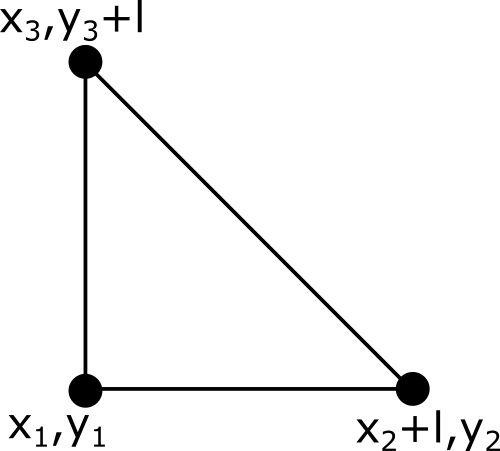
\includegraphics[width=0.8\textwidth]{figure1.png}
\caption{The atomic arrangement.}
\label{figure1}
\end{figure}

\begin{enumerate}[(a)]
\item For a molecule that consists of three identical atoms located at vertices of a $45^{\circ}$ 
right triangle as shown in Figure \ref{figure1}. The atoms have equal spring constants $k$ 
between each atoms. For planer motion we 
define our generalized coordinates by defining the atom with the right angle as $(x_1,y_2)$ 
which implies if the separation distance is $l$ we have $(x_2+l,y_2)$ and $(x_3,x_3+l)$. We
note that all three particles share mass $m$ which makes our kinetic energy
$$T = \frac{1}{2}m\left(\dot{x}_1^2+\dot{x}_2^2+\dot{x}_3^2+\dot{y}_1^2+\dot{y}_2^2+\dot{y}_3^2\right)$$
which if we write $T$ in the form 
$$T = \frac{1}{2}\dot{\eta}_iM_{ij}\dot{\eta}_j$$
we can easily see that $M_{ij} = m\delta_{ij}$ where $\delta_{ij}$ corresponds to the 
identity matrix. For the potential energy we note that it is dependent on the separation 
between the atoms. This is given by the distance formula where we assume that the oscillations
are small along which implies that the separation distance $l$ dominates. This yields 
\begin{align*}
d_{12} &= \sqrt{(l+x_2-x_1)^2+(y_2-y_1)^2} \approx l+x_2-x_1\\
d_{13} &= \sqrt{(x_3-x_1)^2+(l+y_3-y_1)^2} \approx l+y_3-y_1\\
d_{23} &= \sqrt{(x_3-x_2-l)^2+(l+y_3-y_1)^2} \approx \sqrt{2}l - \frac{\sqrt{2}}{2}(x_3-x_2) + \frac{\sqrt{2}}{2}(y_3-y_2)
\end{align*}
So our potential is dependent on the differences between $d$ and the equilibrium length $l$
\begin{align*}
V &= \frac{1}{2}k\left((d_{12}-l)^2 + (d_{13}-l)^2 + (d_{23}-\sqrt{2}l)^2 \right)\\
&= \frac{1}{2}k\left(l+x_2-x_1-1)^2 + (l+y_3-y_1-l)^2 + \left(\sqrt{2}l-\frac{\sqrt{2}}{2}(x_3-x_2)+\frac{\sqrt{2}}{2}(y_3-y_2)-\sqrt{2}l\right)^2 \right)\\
&= \frac{1}{2}k\left((x_2-x_1)^2 + (y_3-y_1)^2 + \frac{1}{2}\left((y_3-y_2)-(x_3-x_2)\frac{}{}\right)^2 \right)\\
&= \frac{1}{2}k\left((x_2-x_1)^2 + (y_3-y_1)^2 + \frac{1}{2}(y_3-y_2)^2 + \frac{1}{2}(x_3-x_2)^2 - (x_3-x_2)(y_3-y_2)\right)\\
\end{align*}
With this potential we can find the matrix elements by
$$V_{ij} = \frac{\partial V}{\partial\eta_i\partial\eta_j}$$
where $\eta_i = (x_1,y_1,x_2,y_2,x_3,y_3)$. We note that this is will create a symmetric 
matrix So we calculate neglecting the common factor of $k$ we find that 
$$\partiald{V}{x_1} = -(x_2-x_1)$$
which allows us to calculate
\begin{align*}
V_{11} &= -\partiald{}{x_1}(x_2-x_1) = 1\\
V_{12} &= -\partiald{}{y_2}(x_2-x_1) = 0 \\
V_{13} &= -\partiald{}{x_2}(x_2-x_1) = -1\\
V_{14}&=V_{15}=V_{16}=0
\end{align*}
Now we see for the first derivative with respect to $y_1$ we have
$$\partiald{V}{y_1} = -(y_3-y_1)$$
which gives us the unique values 
\begin{align*}
V_{22} &= -\partiald{}{y_1}(y_3-y_1) = 1\\
V_{23} &= -\partiald{}{x_2}(y_3-y_1) = 0\\
V_{24} &= -\partiald{}{y_2}(y_3-y_1) = 0\\
V_{25} &= -\partiald{}{x_3}(y_3-y_1) = 0\\
V_{26} &= -\partiald{}{y_3}(y_3-y_1) = -1
\end{align*}
And for $x_2$ we have
$$\partiald{V}{x_2} = (x_2-x_1)-\frac{1}{2}(x_3-x_2)+\frac{1}{2}(y_3-y_2)$$
\begin{align*}
V_{33} &= \partiald{}{x_2}(x_2-x_1)-\frac{1}{2}(x_3-x_2)+\frac{1}{2}(y_3-y_2) = \frac{3}{2}\\
V_{34} &= \partiald{}{y_2}(x_2-x_1)-\frac{1}{2}(x_3-x_2)+\frac{1}{2}(y_3-y_2) = -\frac{1}{2}\\
V_{35} &= \partiald{}{x_3}(x_2-x_1)-\frac{1}{2}(x_3-x_2)+\frac{1}{2}(y_3-y_2) = -\frac{1}{2}\\
V_{36} &= \partiald{}{y_3}(x_2-x_1)-\frac{1}{2}(x_3-x_2)+\frac{1}{2}(y_3-y_2) = \frac{1}{2}
\end{align*}
And for $y_2$
$$\partiald{V}{y_2} = \frac{1}{2}(x_3-x_2)-\frac{1}{2}(y_3-y_2)$$
\begin{align*}
V_{44} &= \partiald{}{y_2}\frac{1}{2}(x_3-x_2)-\frac{1}{2}(y_3-y_2) = \frac{1}{2}\\
V_{45} &= \partiald{}{x_3}\frac{1}{2}(x_3-x_2)-\frac{1}{2}(y_3-y_2) = \frac{1}{2}\\
V_{46} &= \partiald{}{y_3}\frac{1}{2}(x_3-x_2)-\frac{1}{2}(y_3-y_2) = -\frac{1}{2}
\end{align*}
And for $x_3$
$$\partiald{V}{x_3} = \frac{1}{2}(x_3-x_2)-\frac{1}{2}(y_3-y_2)$$
\begin{align*}
V_{55} &= \partiald{}{x_3}\frac{1}{2}(x_3-x_2)-\frac{1}{2}(y_3-y_2) = \frac{1}{2}\\
V_{56} &= \partiald{}{y_3}\frac{1}{2}(x_3-x_2)-\frac{1}{2}(y_3-y_2) = -\frac{1}{2}\\
\end{align*}
And for $y_3$
$$V_{66} = \partiald{^2V}{y_3^2} = \partiald{}{y_3}\frac{1}{2}(y_3-y_2)+(y_3-y_1)-\frac{1}{2}(x_3-x_2) = \frac{3}{2}$$
Combining these into the matrix $\mathbf{V}$ we have
$$\mathbf{V} = k\left(\begin{array}{cccccc}
 1 & 0 & -1 & 0 & 0 & 0 \\
 0 & 1 & 0 & 0 & 0 & -1 \\
 -1 & 0 & \frac{3}{2} & -\frac{1}{2} & -\frac{1}{2} & \frac{1}{2} \\
 0 & 0 & -\frac{1}{2} & \frac{1}{2} & \frac{1}{2} & -\frac{1}{2} \\
 0 & 0 & -\frac{1}{2} & \frac{1}{2} & \frac{1}{2} & -\frac{1}{2} \\
 0 & -1 & \frac{1}{2} & -\frac{1}{2} & -\frac{1}{2} & \frac{3}{2} 
\end{array}\right)$$
We can find the eigenfrequencies by solving
$$-\omega^2M_{ij}+V_{ij}=0$$
Using a numerical methods we find the eigenvalues of this we get
\begin{align*}
\omega_1^2 &= \omega_2^2 = \omega_3^2 = 0\\
\omega_4^2 &= \frac{k}{m}\\
\omega_5^2 &= \frac{2k}{m}\\
\omega_6^2 &= \frac{3k}{m}
\end{align*}
which corresponds to the eigenmodes of motion. We note the three degenerate modes of 
$\omega^2=0$.

\item The three degenerate modes are related to the two translations in $x$ and $y$. The 
final degenerate mode is given by the rotation in the plane. These modes are described by 
the eigenvectors
$$\vec{\eta}_1 = \left(\begin{array}{c}1\\0\\1\\0\\1\\0\end{array}\right)
\qquad\vec{\eta}_2 = \left(\begin{array}{c}0\\1\\0\\1\\0\\1\end{array}\right)
\qquad\vec{\eta}_3 = \left(\begin{array}{c}1/2\\-1/2\\1\\1/2\\-1\\-1\end{array}\right)$$
We note that these modes do not
have vibrational frequency this is why they have a zero value for $\omega^2$. The 
non-degenerate solutions have eigenvectors given by
$$\vec{\eta}_4 = \left(\begin{array}{c}-1\\-1\\0\\1\\1\\0\end{array}\right)
\qquad\vec{\eta}_5 = \left(\begin{array}{c}1\\-1\\-1\\0\\0\\1\end{array}\right)
\qquad\vec{\eta}_6 = \left(\begin{array}{c}-1/2\\-1/2\\1\\-1/2\\-1/2\\1\end{array}\right)$$
We see that $\omega^2_4$ is the vibrational mode along the $x$ and $y$ or along the 
direction of the legs. Note that $\omega^2_5$ is vibration along the hypotenuse and the 
$\omega^2_6$ is the vibrational mode that expands and contracts the triangle as a whole. Note
that each vibrational mode corresponds to a single spring vibration and double spring then a
triple spring which explains the factors of $1$, $2$, and $3$ in the eigenfrequencies.
\end{enumerate}

\pagebreak

\section{Problem \#4}
\begin{figure}
\centering
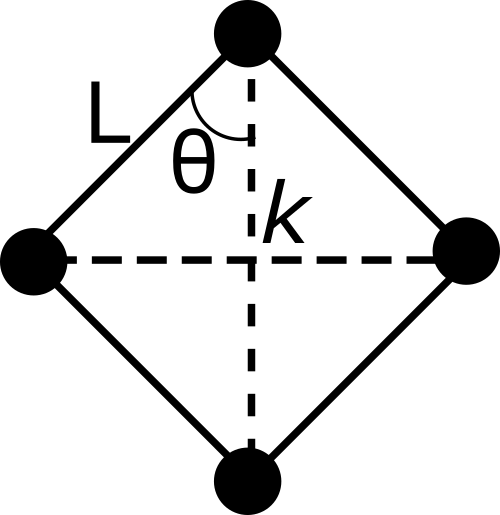
\includegraphics[width=0.8\textwidth]{figure2.png}
\caption{Four masses on a rhombus.}
\label{figure2}
\end{figure}
We can see that the system shown in Figure \ref{figure2} of four massless rods of length $L$ are hinged together at their
ends to form a rhombus. At each corner there is a particle of mass $m$ with a spring attached
to opposite corners with a spring constant, $k$. By looking at the system a vibration in
one spring will constrain the vibration in the other. We define this coordinate as the angle, $\theta$
between a spring and the nearest rod. Which gives
$$x = L\cos\theta\qquad y = L\sin\theta$$
and the first derivative yields
$$\dot{x} = -L\sin\theta\dot{\theta}\qquad \dot{y} = L\cos\theta\dot{\theta}$$
Now we can find the kinetic energy by noting that the particles are restricted to move only 
in the direction of the springs. This simplifies the problems a great deal as the opposite 
particle will have mirrored movement.
\begin{align*}
T &= \frac{1}{2}m(2\dot{x}^2+2\dot{y}^2)\\
&= m(L^2\sin^2\theta\dot{\theta}^2+L^2\cos^2\theta\dot{\theta}^2)\\
&= mL^2\dot{\theta}^2
\end{align*}
Note the factors of $2$ arise from the fact that we have two particles moving in $x$ and $y$
And for displacements from the equilibrium length $\sqrt{2}L$ give the potential energy
\begin{align*}
V &= \frac{1}{2}k\left(\frac{}{}(\sqrt{2}L-2x)^2+(\sqrt{2}L-2y)^2\right)\\
&= \frac{1}{2}k\left(\frac{}{}(\sqrt{2}L-2L\cos\theta)^2+(\sqrt{2}L-2L\sin\theta)^2\right)\\
&= \frac{1}{2}kL^2\left(\frac{}{}(\sqrt{2}-2\cos\theta)^2+(\sqrt{2}-2\sin\theta)^2\right)\\
&= \frac{1}{2}kL^2\left(\frac{}{}2+4\cos^2\theta-4\sqrt{2}\cos\theta+2-4\sin^2\theta+4\sqrt{2}\sin\theta\right)\\
&= kL^2\left(\frac{}{}4-2\sqrt{2}(\sin\theta+\cos\theta)\right)\\
&= kL^2\left(\frac{}{}4-2\sqrt{2}\sqrt{2}\sin(\theta+\pi/4)\right)\\
&= 4kL^2\left(\frac{}{}1-\sin(\theta+\pi/4)\right)
\end{align*}
This yields the Lagrangian 
$$L = mL^2\dot{\theta}^2 -4kL^2\left(\frac{}{}1-\sin(\theta+\pi/4)\right)$$
Now we can calculate the equations of motion by
\begin{align*}
\frac{d}{dt}\partiald{L}{\dot{\theta}} - \partiald{L}{\theta} &= 0\\
&\Downarrow\\
\frac{d}{dt}(2mL^2\dot{\theta}) + 4kL^2\cos(\theta+\pi/4) &= 0\\
2mL^2\ddot{\theta} &= -4kL^2\cos(\theta+\pi/4)\\
&\Downarrow\\
\ddot{\theta} &= -\frac{4kL^2}{2mL^2}\cos(\theta+\pi/4)\\
\ddot{\theta} &= -\frac{2k}{m}\cos(\theta+\pi/4)
\end{align*}
We can take this equation of motion for a small oscillation by noting that the equilibrium 
is when the rhombus is a square which is at $\theta = \pi/4+\delta\theta$ so we have
$$\cos(\theta+\pi/4) = \cos(\delta\theta+\pi/2) = \sin(\delta\theta) = \delta\theta+\scrO(\delta\theta^2)$$ 
This reduces our equation of motion into the simple harmonic motion given by
$$\ddot{\delta\theta} = -\frac{2k}{m}\delta\theta$$
which we can quickly see gives a frequency of small oscillation
$$\omega^2 = \frac{2k}{m}$$

\end{document}

